\documentclass[11pt]{article}

\usepackage[T1]{fontenc}
\usepackage[utf8]{inputenc}
\usepackage{lmodern}
\usepackage{microtype}
\usepackage[a4paper,margin=27mm,headheight=15pt]{geometry}
\usepackage{amsmath,amssymb,mathtools}
\usepackage{amsthm}
\usepackage{booktabs,longtable,array}
\usepackage{enumitem}
\usepackage{graphicx}
\usepackage{xcolor}
\usepackage{listings}
\usepackage{caption}
\usepackage{fancyhdr}
\usepackage{xurl}
\usepackage{hyperref}
\usepackage[nameinlink,capitalize,noabbrev]{cleveref}

\hypersetup{
  colorlinks=true,
  linkcolor=blue!45!black,
  citecolor=green!35!black,
  urlcolor=blue!55!black,
  pdftitle={Diagonal Polynomials and Dyadic Block Geometry in Repeated Thue--Morse Prefix Summation},
  pdfauthor={Prepared for Vladimir Reshetnikov}
}

\pagestyle{fancy}
\fancyhf{}
\fancyhead[L]{Repeated Thue--Morse summation}
\fancyhead[R]{Diagonal polynomials}
\fancyfoot[C]{\thepage}

\allowdisplaybreaks
\setlength{\parindent}{0pt}
\setlength{\parskip}{0.55em}
\setcounter{tocdepth}{2}
\setlength{\emergencystretch}{2em}

\newtheorem{theorem}{Theorem}[section]
\newtheorem{proposition}[theorem]{Proposition}
\newtheorem{corollary}[theorem]{Corollary}
\newtheorem{lemma}[theorem]{Lemma}
\newtheorem{conjecture}[theorem]{Conjecture}
\theoremstyle{definition}
\newtheorem{definition}[theorem]{Definition}
\newtheorem{algorithm}[theorem]{Algorithm}
\theoremstyle{remark}
\newtheorem{remark}[theorem]{Remark}
\newtheorem{example}[theorem]{Example}

\newcommand{\N}{\mathbb N}
\newcommand{\Z}{\mathbb Z}
\newcommand{\Q}{\mathbb Q}
\newcommand{\eps}{\varepsilon}
\newcommand{\K}{\mathcal K}
\newcommand{\Sgen}{\mathcal S}
\newcommand{\A}{\mathcal A}
\newcommand{\Diag}{D}
\newcommand{\coeff}[2]{[z^{#1}]\,#2}
\newcommand{\rising}[2]{#1^{\overline{#2}}}
\newcommand{\wt}{\operatorname{wt}_2}
\newcommand{\cont}{\operatorname{cont}}
\newcommand{\vTwo}{\nu_2}
\newcommand{\Up}{\operatorname{up}}
\newcommand{\stirlingone}[2]{\genfrac{[}{]}{0pt}{}{#1}{#2}}

\definecolor{codebg}{RGB}{247,247,247}
\definecolor{codeframe}{RGB}{210,210,210}
\definecolor{codecomment}{RGB}{70,110,70}
\definecolor{codekeyword}{RGB}{40,60,150}

\lstdefinelanguage{Wolfram}{
  morekeywords={ClearAll,Module,Sum,Product,Table,Expand,Factor,FullSimplify,
  Binomial,Factorial,Quotient,QuotientRemainder,Mod,Range,Select,Times,
  IntegerExponent,IntegerLength,SeriesCoefficient,Coefficient,PossibleZeroQ,
  ThueMorse,With,If,And,Flatten,MapThread,Total},
  sensitive=true,
  morecomment=[s]{(*}{*)},
  morestring=[b]"
}

\lstset{
  basicstyle=\ttfamily\small,
  keywordstyle=\color{codekeyword}\bfseries,
  commentstyle=\color{codecomment},
  stringstyle=\color{purple!60!black},
  backgroundcolor=\color{codebg},
  frame=single,
  rulecolor=\color{codeframe},
  breaklines=true,
  columns=fullflexible,
  keepspaces=true,
  showstringspaces=false,
  aboveskip=0.8em,
  belowskip=0.8em
}

\title{\textbf{Diagonal Polynomials and Dyadic Block Geometry\\
  in Repeated Thue--Morse Prefix Summation}\\[0.4em]
  \large Exact formulas, denominator laws, rational roots, and fast Wolfram Language evaluation}
\author{Prepared for Vladimir Reshetnikov}
\date{3 September 2026}

\begin{document}
\maketitle

\begin{abstract}
Let \(\eps_m=(-1)^{\wt(m)}\) be the signed Thue--Morse sequence and let
\(\sigma_r\) be its \(r\)-fold inclusive prefix sum.  We analyze the
Wolfram Language table in the prompt, whose recursive step convolves one row
with the weights \(1,2,3,\ldots\).  The first structural result is the exact
identification
\[
 s_{n,k}=\sigma_{2n+1}(k-n-1),
\]
where negative arguments of \(\sigma_r\) are interpreted as zero.  Thus one
row step performs two further prefix summations and shifts the column by one.
For a fixed diagonal offset \(d\geq1\), write \(q=d-1\).  Then
\[
 s_{n,n+d}=\Diag_q(n),
 \qquad
 \boxed{
 \Diag_q(x)=\sum_{j=0}^{\lfloor q/2\rfloor}
   \eps_j\binom{2x+q-2j-1}{q-2j}}
\]
with the binomial understood polynomially.  Equivalently,
\[
 \sum_{q\geq0}\Diag_q(x)z^q
  =\frac{\K(z^2)}{(1-z)^{2x}},
 \qquad
 \Diag_q(x)=\sum_{j=0}^{\lfloor q/2\rfloor}
 \eps_j\frac{\rising{(2x)}{q-2j}}{(q-2j)!}.
\]
This is the requested general shape: a sparse, Thue--Morse-signed expansion
in rising factorials of degrees \(q,q-2,q-4,\ldots\).  It immediately gives
\(\deg\Diag_q=q\), leading coefficient \(2^q/q!\), exact monomial
coefficients through unsigned Stirling numbers, and fast evaluation in
\(O(q)\) exact-arithmetic terms.

We also prove several finer facts.  The least positive integer clearing all
monomial coefficients is
\[
 \frac{q!}{2^{\min(\vTwo(q!),\lceil q/2\rceil)}}.
\]
Every rational root of \(\Diag_q\) is an integer or half-integer.  All
nonnegative rational roots are classified exactly: \(x=m/2\), \(m\geq0\),
is a root if and only if
\[
 q\bmod 2^{m+1}\;\geq\;2^{m+1}-(m+1).
\]
Finally, a finite positive pulse polynomial describes every row.  Its
coefficients are positive, palindromic, unimodal, have an exactly flat
central plateau, and repeat in dyadic blocks with Thue--Morse signs.  This
single block theorem explains the sign, reflection, complement, zero-window,
and peak-height clauses in the supplied Wolfram Language program.
\end{abstract}

\tableofcontents
\newpage

\section{Introduction and scope}

The repository \cite{ProveIt} develops a detailed connection between the
signed Thue--Morse sequence, iterated prefix sums, finite product
approximants, the Rvachev \(\operatorname{up}\)-function, and the Fabius
function.  In the notation used there, the basic discrete objects are the
inclusive prefix sums
\[
 \sigma_0(m)=\eps_m,
 \qquad
 \sigma_{r+1}(m)=\sum_{j=0}^{m}\sigma_r(j),
\]
and their formal generating series satisfy
\[
 \sum_{m\geq0}\sigma_r(m)z^m
   =\frac{\K(z)}{(1-z)^r},
 \qquad
 \K(z)=\sum_{m\geq0}\eps_mz^m
       =\prod_{j\geq0}(1-z^{2^j}).
\]
The infinite product is interpreted coefficientwise in the formal setting:
only finitely many factors affect any specified coefficient.  The repository
also identifies the finite positive product
\[
 \prod_{j=1}^{r-1}(1+z+\cdots+z^{2^j-1})
\]
with the first dyadic coefficient block of the order-\(r\) prefix row.
Those facts are our starting point.

The table in the prompt is not indexed directly by prefix order.  Its row
recurrence is
\begin{equation}
 s_{n,k}=\sum_{j=0}^{k-1}(k-j)s_{n-1,j},                 \label{eq:user-rec}
\end{equation}
which is a convolution by \(1,2,3,\ldots\).  The initial explicit formulas
show that values on the lines \(k=n+d\) are polynomial in \(n\), but the
reason, the general polynomial, and the arithmetic of its coefficients are
not apparent from the code alone.

This article has four main goals.

\begin{enumerate}[leftmargin=2.2em]
\item Identify the entire two-dimensional table with a shifted subsequence of
the iterated prefix-sum array.
\item Derive a closed polynomial formula for every diagonal and explain its
basis, degree, leading terms, denominators, and root factors.
\item Prove a complete dyadic block description of every row and use it to
explain all acceleration clauses in the supplied program.
\item Give compact Wolfram Language routines for direct evaluation,
polynomial generation, root extraction, and independent verification.
\end{enumerate}

The proofs below are self-contained.  Statements already present in the
repository are cited as inputs; the table identification, diagonal theory,
coefficient-content theorem, rational-root restriction, and half-grid root
classification are derived here from those inputs.  The accompanying Python
program performs independent exact checks but is not used as a substitute
for proof.

\section{Signed Thue--Morse prefixes}

\subsection{Signs, prefix sums, and conventions}

Let \(\wt(m)\) denote the number of ones in the binary expansion of
\(m\in\N\).  This is the standard signed form of the Thue--Morse
sequence \cite{AlloucheShallit}; define
\begin{equation}
 \eps_m=(-1)^{\wt(m)}.                                      \label{eq:eps-def}
\end{equation}
The two elementary binary recurrences are
\begin{equation}
 \eps_{2m}=\eps_m,
 \qquad
 \eps_{2m+1}=-\eps_m.                                      \label{eq:eps-binary}
\end{equation}
We use inclusive prefix sums.

\begin{definition}[Iterated inclusive prefixes]
For \(r,m\in\N\), define
\begin{equation}
 \sigma_0(m)=\eps_m,
 \qquad
 \sigma_{r+1}(m)=\sum_{j=0}^{m}\sigma_r(j).                \label{eq:sigma-def}
\end{equation}
For convenience in shifted formulas, set \(\sigma_r(m)=0\) whenever
\(m<0\).
\end{definition}

The inclusive convention gives
\begin{equation}
 \sigma_{r+1}(m+1)-\sigma_{r+1}(m)=\sigma_r(m+1).           \label{eq:sigma-diff}
\end{equation}
The standard hockey-stick argument yields the explicit binomial convolution.

\begin{proposition}[Binomial convolution]
For \(r\geq1\) and \(m\geq0\),
\begin{equation}
 \sigma_r(m)=\sum_{a=0}^{m}
   \binom{m-a+r-1}{r-1}\eps_a.                             \label{eq:sigma-conv}
\end{equation}
\end{proposition}

\begin{proof}
For \(r=1\), every binomial coefficient is \(1\), so the formula is the
ordinary prefix sum.  If it holds at order \(r\), then
\begin{align*}
 \sigma_{r+1}(m)
 &=\sum_{j=0}^{m}\sum_{a=0}^{j}
      \binom{j-a+r-1}{r-1}\eps_a \\
 &=\sum_{a=0}^{m}\eps_a
      \sum_{u=0}^{m-a}\binom{u+r-1}{r-1} \\
 &=\sum_{a=0}^{m}\binom{m-a+r}{r}\eps_a,
\end{align*}
which is the next order by the hockey-stick identity.
\end{proof}

\subsection{Formal generating series}

Set
\begin{equation}
 \K(z)=\sum_{m\geq0}\eps_mz^m,
 \qquad
 \Sgen_r(z)=\sum_{m\geq0}\sigma_r(m)z^m.                  \label{eq:series-def}
\end{equation}
From \cref{eq:sigma-def}, multiplication by \((1-z)^{-1}\) performs one
inclusive prefix sum, hence
\begin{equation}
 \Sgen_r(z)=\frac{\K(z)}{(1-z)^r}.                         \label{eq:sigma-gf}
\end{equation}
The binary recurrences \cref{eq:eps-binary} give the Mahler identity
\begin{equation}
 \K(z)=(1-z)\K(z^2),                                      \label{eq:K-mahler}
\end{equation}
and iteration gives the coefficientwise product
\begin{equation}
 \K(z)=\prod_{j\geq0}(1-z^{2^j}).                         \label{eq:K-product}
\end{equation}
Equations \cref{eq:sigma-conv,eq:sigma-gf,eq:K-mahler,eq:K-product} are the
precise discrete ingredients used throughout the rest of the article.

\section{The two-dimensional table}

\subsection{One row step equals two prefix sums}

The weighted kernel in \cref{eq:user-rec} has generating series
\begin{equation}
 \sum_{h\geq1}h z^h=\frac{z}{(1-z)^2}.                     \label{eq:kernel-gf}
\end{equation}
Thus one row step multiplies a row series by \(z(1-z)^{-2}\): the factor
\((1-z)^{-2}\) performs two prefix summations and the factor \(z\) shifts
one column to the right.  This observation completely identifies the table.

\begin{theorem}[Exact table identification]
For all \(n,k\in\N\), the table computed by the supplied rules satisfies
\begin{equation}
 \boxed{s_{n,k}=\sigma_{2n+1}(k-n-1).}                     \label{eq:table-sigma}
\end{equation}
Consequently its row generating series is
\begin{equation}
 T_n(z):=\sum_{k\geq0}s_{n,k}z^k
  =\frac{z^{n+1}\K(z)}{(1-z)^{2n+1}}
  =\frac{z^{n+1}\K(z^2)}{(1-z)^{2n}}.                     \label{eq:row-gf}
\end{equation}
\end{theorem}

\begin{proof}
The row \(n=0\) in the code is zero at even columns and equals
\(\eps_a\) at column \(2a+1\).  Indeed, the sign-block rule reduces every
odd column \(2a+1\) to the value at column \(1\), while every even column
reduces to column \(0\).  On the other hand,
\[
 \sigma_1(2a)=\eps_a,
 \qquad
 \sigma_1(2a+1)=0,
\]
because adjacent Thue--Morse signs cancel.  Therefore
\(s_{0,k}=\sigma_1(k-1)\), and
\[
 T_0(z)=z\Sgen_1(z)=\frac{z\K(z)}{1-z}.
\]

Now assume the formula for row \(n-1\).  Multiplying by the kernel series
\cref{eq:kernel-gf} gives
\[
 T_n(z)=\frac{z}{(1-z)^2}T_{n-1}(z)
 =\frac{z^{n+1}\K(z)}{(1-z)^{2n+1}}.
\]
The coefficient of \(z^k\) is
\(\sigma_{2n+1}(k-n-1)\), proving \cref{eq:table-sigma}.

For a direct index proof, put \(q=k-n-1\).  The recurrence right side is
\begin{align*}
 \sum_{j=0}^{k-1}(k-j)s_{n-1,j}
 &=\sum_{i=0}^{q}(q+1-i)\sigma_{2n-1}(i)\\
 &=\sum_{u=0}^{q}\sum_{i=0}^{u}\sigma_{2n-1}(i)
 =\sigma_{2n+1}(q),
\end{align*}
which is exactly two inclusive prefix summations.
Finally, \cref{eq:K-mahler} gives the second expression in
\cref{eq:row-gf}.
\end{proof}

The first rows illustrate both the initial zero triangle and the rapid
formation of a positive pulse.
\begin{center}
\small
\setlength{\tabcolsep}{3.6pt}
\begin{tabular}{c|rrrrrrrrrrrrrrrrr}
\toprule
\(n\backslash k\)&0&1&2&3&4&5&6&7&8&9&10&11&12&13&14&15&16\\
\midrule
0&0&1&0&-1&0&-1&0&1&0&-1&0&1&0&1&0&-1&0\\
1&0&0&1&2&2&2&1&0&0&0&-1&-2&-2&-2&-1&0&0\\
2&0&0&0&1&4&9&16&24&32&40&48&55&60&63&64&64&64\\
3&0&0&0&0&1&6&20&50&104&190&316&490&719&1008&1360&1776&2256\\
\bottomrule
\end{tabular}
\end{center}

\subsection{Bivariate generating functions}

Summing \cref{eq:row-gf} over \(n\) gives a compact generating function for
the whole table.

\begin{corollary}[Full table series]
As a formal power series in \(u\), with coefficients that are formal power
series in \(z\),
\begin{equation}
 \sum_{n,k\geq0}s_{n,k}u^nz^k
 =\frac{z(1-z)\K(z)}{(1-z)^2-uz}.                          \label{eq:full-bivar}
\end{equation}
After shifting to the diagonal coordinate \(q=k-n-1\),
\begin{equation}
 \sum_{n,q\geq0}s_{n,n+q+1}u^nz^q
 =\frac{(1-z)^2\K(z^2)}{(1-z)^2-u}.                        \label{eq:diag-bivar}
\end{equation}
\end{corollary}

\begin{proof}
Both formulas are geometric sums.  For example,
\[
 \sum_{n\geq0}u^nT_n(z)
 =\frac{z\K(z)}{1-z}
   \sum_{n\geq0}\left(\frac{uz}{(1-z)^2}\right)^n,
\]
which simplifies to \cref{eq:full-bivar}.  Removing the shift
\(z^{n+1}\) first gives \cref{eq:diag-bivar}.
\end{proof}

\section{Exact dyadic block geometry of every row}

\subsection{The positive pulse polynomial}

For an order \(r\geq1\), define
\begin{equation}
 \A_r(z)=\prod_{j=1}^{r-1}(1+z+\cdots+z^{2^j-1})
        =\sum_{b=0}^{2^r-r-1}a_{r,b}z^b.                  \label{eq:A-def}
\end{equation}
The product is empty when \(r=1\), so \(\A_1=1\).  Splitting the first
\(r\) factors from \(\K\) gives an exact block factorization.

\begin{theorem}[Signed block factorization]
For every \(r\geq1\),
\begin{equation}
 \frac{\K(z)}{(1-z)^r}=\A_r(z)\K(z^{2^r}).                 \label{eq:block-factor}
\end{equation}
Consequently, if \(q=a2^r+b\) with \(a\geq0\) and
\(0\leq b<2^r\), then
\begin{equation}
 \boxed{\sigma_r(q)=\eps_a a_{r,b},}                      \label{eq:block-law}
\end{equation}
where \(a_{r,b}=0\) for \(b>2^r-r-1\).
\end{theorem}

\begin{proof}
From the iterated Mahler identity,
\[
 \K(z)=\left(\prod_{j=0}^{r-1}(1-z^{2^j})\right)\K(z^{2^r}).
\]
The factor \(j=0\) is \(1-z\); for each \(1\leq j<r\), divide
\(1-z^{2^j}\) by \(1-z\).  This yields \cref{eq:block-factor}.
Since \(\deg\A_r=2^r-r-1<2^r\), the coefficient of
\(z^{a2^r+b}\) comes from the unique product of \(\eps_a z^{a2^r}\)
in \(\K(z^{2^r})\) and \(a_{r,b}z^b\) in \(\A_r\).
\end{proof}

This sharpens the usual terminal-zero statement: it identifies every zero
and every nonzero value in every block.

\begin{corollary}[Complete zero and sign criterion]
For \(q=a2^r+b\), \(0\leq b<2^r\),
\begin{align}
 \sigma_r(q)=0
 &\iff b\geq2^r-r,                                        \label{eq:zero-criterion}\\
 \operatorname{sgn}\sigma_r(q)
 &=\eps_a\quad\text{whenever }\sigma_r(q)\ne0.            \label{eq:sign-criterion}
\end{align}
Thus every dyadic block ends in exactly \(r\) zeros, and each nonzero block
is a positive pulse multiplied by one Thue--Morse sign.
\end{corollary}

\begin{proof}
Every coefficient of \(\A_r\) between degrees \(0\) and
\(2^r-r-1\) is strictly positive.  One way to see this is the tuple
interpretation in \cref{prop:pulse-shape} below.  Outside that range the
coefficient is zero.  Apply \cref{eq:block-law}.
\end{proof}

\subsection{Shape, mass, plateau, and moments}

\begin{proposition}[Complete shape of the positive pulse]\label{prop:pulse-shape}
The coefficients of \(\A_r\) have the following properties.

\begin{enumerate}[label=(\roman*),leftmargin=2.4em]
\item \(a_{r,b}\) counts tuples
\[
 (u_1,\ldots,u_{r-1}),\qquad
 0\leq u_j\leq2^j-1,\qquad \sum_{j=1}^{r-1}u_j=b.
\]
Hence every coefficient on the full support
\(0\leq b\leq2^r-r-1\) is a positive integer.

\item The sequence is palindromic:
\begin{equation}
 a_{r,b}=a_{r,2^r-r-1-b}.                                 \label{eq:pulse-pal}
\end{equation}

\item Its total mass is
\begin{equation}
 \sum_b a_{r,b}=\A_r(1)=2^{\binom r2}.                    \label{eq:pulse-mass}
\end{equation}

\item It is nondecreasing to the center, constant on exactly \(r\)
consecutive central indices, and nonincreasing thereafter.  The maximum is
\begin{equation}
 \max_b a_{r,b}=2^{\binom{r-1}{2}},                        \label{eq:pulse-peak}
\end{equation}
and it occurs for
\begin{equation}
 2^{r-1}-r\leq b\leq2^{r-1}-1.                            \label{eq:pulse-plateau}
\end{equation}

\item After normalization by \(2^{\binom r2}\), the coefficients form the
probability mass function of
\[
 U_1+\cdots+U_{r-1},
 \qquad U_j\sim\operatorname{Unif}\{0,1,\ldots,2^j-1\},
\]
with independent summands.  Therefore
\begin{align}
 \mathbb E\sum U_j&=\frac{2^r-r-1}{2},                    \label{eq:pulse-mean}\\
 \operatorname{Var}\sum U_j&=\frac{4^r-3r-1}{36}.         \label{eq:pulse-var}
\end{align}
\end{enumerate}
\end{proposition}

\begin{proof}
The tuple interpretation is obtained by choosing one monomial from each
factor in \cref{eq:A-def}.  The sum of the upper bounds is
\(\sum_{j=1}^{r-1}(2^j-1)=2^r-r-1\), and convolution of integer intervals
has no gaps.  Each factor is palindromic, proving (ii).  Evaluating the
factors at \(z=1\) gives
\(\prod_{j=1}^{r-1}2^j=2^{\binom r2}\), proving (iii).

For (iv), put \(H=2^{r-1}\).  Then
\[
 \A_r(z)=\A_{r-1}(z)(1+z+\cdots+z^{H-1}).
\]
The degree of \(\A_{r-1}\) is \(H-r\).  For \(b<H\),
\begin{equation}
 a_{r,b}=\sum_{u=0}^{\min(b,H-r)}a_{r-1,u}.                \label{eq:pulse-prefix}
\end{equation}
This sum increases strictly until \(b=H-r\), then equals the full mass
\(\A_{r-1}(1)=2^{\binom{r-1}{2}}\) through \(b=H-1\).
Palindromy supplies the descending half.  The plateau contains
\(H-1-(H-r)+1=r\) indices.

For (v), divide every factor by its value \(2^j\) at \(1\).  The mean of
\(U_j\) is \((2^j-1)/2\), and its variance is
\(((2^j)^2-1)/12\).  Summing and using geometric-series formulas gives
\cref{eq:pulse-mean,eq:pulse-var}.
\end{proof}

\begin{figure}[htbp]
\centering
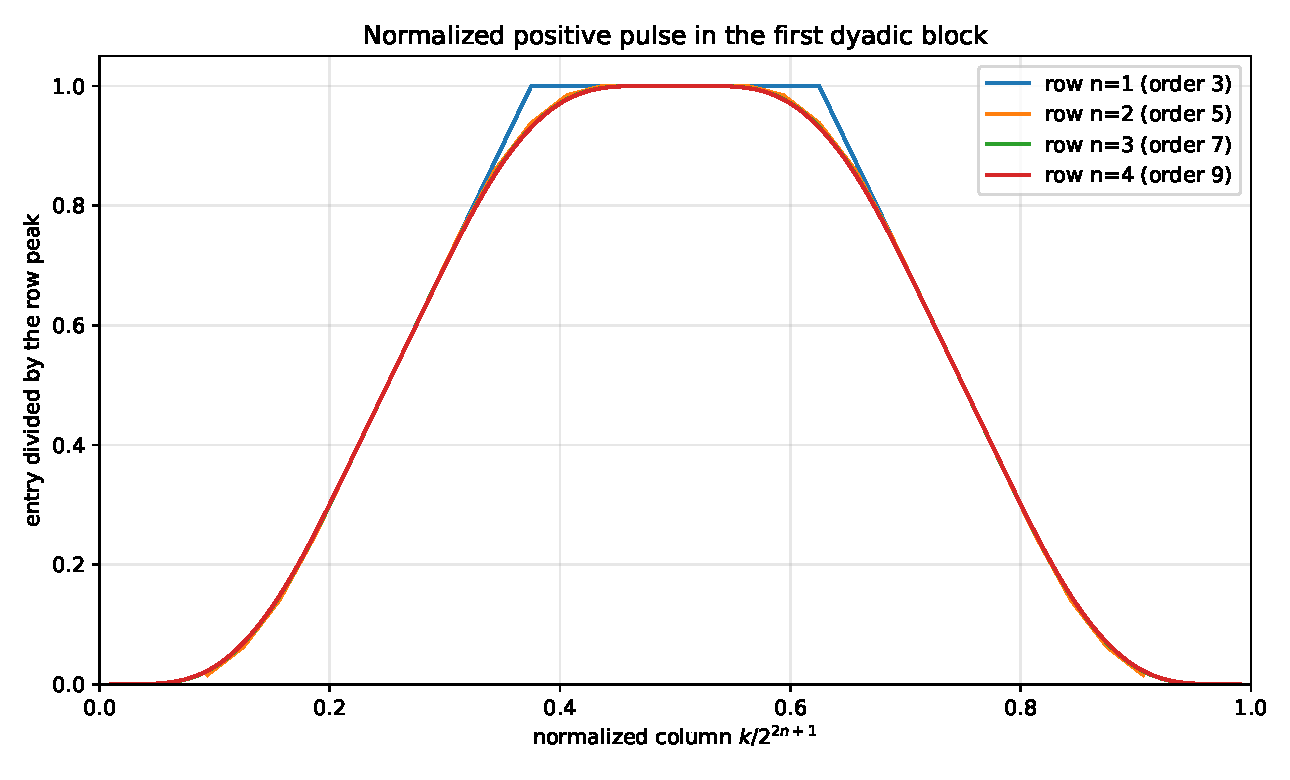
\includegraphics[width=0.9\textwidth]{figures/normalized_row_pulses.pdf}
\caption{The positive pulse in the first dyadic block of rows
\(n=1,2,3,4\), divided by its exact peak
\(2^{\binom{2n}{2}}\) and plotted against normalized column
\(k/2^{2n+1}\).  The pulse is centered at \(1/2\); the exact central plateau
has \(2n+1\) lattice points.}
\label{fig:pulses}
\end{figure}

\subsection{Specialization to the supplied table}

Put
\begin{equation}
 r=2n+1,
 \qquad B=2^r=2^{2n+1},
 \qquad H=2^{r-1}=2^{2n},
 \qquad c=n+1.                                             \label{eq:row-params}
\end{equation}
By \cref{eq:table-sigma}, the shifted coordinate is \(q=k-c\).  Combining
this shift with \cref{eq:block-law} gives a complete row formula directly in
the code's column coordinate.

\begin{theorem}[Exact first-block pulse and signed repetition]
Write \(k=aB+b\), where \(0\leq b<B\).  Then
\begin{equation}
 s_{n,k}=
 \begin{cases}
 0, & 0\leq b\leq n,\\
 \eps_a\,a_{2n+1,b-n-1},&n+1\leq b\leq B-n-1,\\
 0,&B-n\leq b<B.
 \end{cases}                                               \label{eq:row-block-k}
\end{equation}
Inside every block the nonzero pulse is palindromic about \(k=aB+H\), has
height
\begin{equation}
 M_n=2^{\binom{2n}{2}},                                    \label{eq:Mn}
\end{equation}
and has a flat top at the \(2n+1\) columns
\begin{equation}
 aB+H-n,\ldots,aB+H+n.                                    \label{eq:row-plateau}
\end{equation}
Adjacent blocks are separated by a zero run of length \(2n+1\), and the
sign of block \(a\) is \(\eps_a\).
\end{theorem}

\begin{proof}
If \(b\geq c\), then
\(q=aB+(b-c)\), so \cref{eq:block-law} applies with the same block index
\(a\).  If \(b<c\), the shifted residue lies in the terminal zero window of
the preceding \(q\)-block; both sides of \cref{eq:row-block-k} are zero.
The end of the support follows from
\(b-c\leq B-(2n+1)-1\), which is equivalent to
\(b\leq B-n-1\).  The remaining claims are translations of
\cref{eq:pulse-peak,eq:pulse-plateau}.
\end{proof}

The code's three non-polynomial acceleration rules now become transparent.

\begin{corollary}[The sign, reflection, and complement rules]
With \(B,H,M_n\) as in \cref{eq:row-params,eq:Mn}, the following identities
hold whenever the displayed arguments are nonnegative:
\begin{align}
 s_{n,aB+b}&=\eps_a s_{n,b} &&\text{on the nonzero part of a block},
                                                               \label{eq:code-sign}\\
 s_{n,k}&=s_{n,B-k},                                           \label{eq:code-reflect}\\
 s_{n,k}&=M_n-s_{n,H-k}\qquad(0\leq k\leq H).                       \label{eq:code-complement}
\end{align}
The guards in the prompt choose subranges of
\cref{eq:code-reflect,eq:code-complement} on which the new argument is
strictly smaller, thereby ensuring rapid recursive reduction.
\end{corollary}

\begin{proof}
The sign rule is \cref{eq:row-block-k}.  For reflection, put
\(D=\deg\A_{2n+1}=B-2n-2\).  The pulse coordinate at column \(k\) is
\(k-c\), while the pulse coordinate at \(B-k\) is
\(B-k-c=D-(k-c)\).  Thus \cref{eq:code-reflect} is precisely the
palindromy \cref{eq:pulse-pal}.

For the complement, let \(D_-=H-(2n+1)\), the degree of
\(\A_{2n}\).  The prefix-sum representation \cref{eq:pulse-prefix} and
palindromy of \(\A_{2n}\) give
\[
 a_{2n+1,q}=M_n-a_{2n+1,D_--1-q}.
\]
Since \(D_--1-(k-c)=H-k-c\), this is exactly
\cref{eq:code-complement} after translating back to columns.
\end{proof}

Thus the apparently unrelated constants and cut points in the original code
are forced by one finite product: \(B\) is its repetition period,
\(H\) its center, \(M_n\) its plateau height, and the two reflections are
ordinary coefficient palindromy and cumulative-complement symmetry.

\section{The general diagonal polynomial}

\subsection{Definition and three equivalent formulas}

Fix an offset \(d\geq1\), and write
\begin{equation}
 q=d-1.                                                      \label{eq:q-d}
\end{equation}
The diagonal in the prompt is \(k=n+d=n+q+1\).  By
\cref{eq:table-sigma}, its value is \(\sigma_{2n+1}(q)\).  For fixed \(q\),
the prefix order varies with \(n\), and the binomial convolution makes the
polynomial dependence explicit.

\begin{theorem}[Diagonal polynomial theorem]\label{thm:diag-main}
For every \(q\geq0\), there is a unique polynomial
\(\Diag_q(x)\in\Q[x]\) such that
\begin{equation}
 s_{n,n+q+1}=\Diag_q(n)\qquad(n\in\N).                     \label{eq:diag-interp}
\end{equation}
It has the equivalent formulas
\begin{align}
 \Diag_q(x)
 &=\sum_{a=0}^{q}\eps_a
   \binom{2x+q-a}{q-a},                                    \label{eq:diag-dense}\\
 &=\sum_{j=0}^{\lfloor q/2\rfloor}\eps_j
   \binom{2x+q-2j-1}{q-2j},                               \label{eq:diag-sparse}\\
 &=\sum_{j=0}^{\lfloor q/2\rfloor}\eps_j
   \frac{\rising{(2x)}{q-2j}}{(q-2j)!}.                   \label{eq:diag-rising}
\end{align}
Its ordinary generating function in the diagonal index is
\begin{equation}
 \boxed{
 \sum_{q\geq0}\Diag_q(x)z^q
  =\frac{\K(z^2)}{(1-z)^{2x}}
  =\frac{\displaystyle\prod_{j\geq1}(1-z^{2^j})}
         {(1-z)^{2x}}.}                                    \label{eq:diag-gf}
\end{equation}
For a fixed coefficient \(q\), the product in \cref{eq:diag-gf} may be
truncated after the last \(2^j\leq q\).
\end{theorem}

\begin{proof}
Insert \(r=2n+1\) and \(m=q\) in the binomial convolution
\cref{eq:sigma-conv}:
\[
 s_{n,n+q+1}=\sigma_{2n+1}(q)
 =\sum_{a=0}^{q}\eps_a\binom{q-a+2n}{2n}
 =\sum_{a=0}^{q}\eps_a\binom{2n+q-a}{q-a}.
\]
Replacing \(n\) by an indeterminate \(x\) gives
\cref{eq:diag-dense}; each summand is a polynomial, so existence follows.
The term \(a=0\) has degree \(q\) and every other term has smaller degree,
which also proves uniqueness from infinitely many values at
\(n=0,1,2,\ldots\).

Alternatively, use the second row-series form in \cref{eq:row-gf}.  The
coefficient at the shifted column is
\[
 \Diag_q(n)=\coeff{q}{\frac{\K(z^2)}{(1-z)^{2n}}}.
\]
The coefficient of \(z^{2j}\) in \(\K(z^2)\) is \(\eps_j\), while
\[
 \coeff{m}{(1-z)^{-2x}}
 =\binom{2x+m-1}{m}
 =\frac{\rising{(2x)}m}{m!}.
\]
Convolution gives \cref{eq:diag-sparse,eq:diag-rising}, and collecting all
coefficients gives \cref{eq:diag-gf}.
\end{proof}

\begin{remark}[The requested ``general shape'']
Formula \cref{eq:diag-rising} is more informative than a monomial expansion.
The degrees that occur in the natural rising-factorial basis are precisely
\[
 q,q-2,q-4,\ldots,
\]
and their signs are the initial Thue--Morse signs
\(\eps_0,\eps_1,\eps_2,\ldots\).  Thus the \(d\)-th diagonal polynomial is
not an isolated interpolation accident: it is the coefficient sequence of
one fixed lacunary product multiplied by the negative-binomial family
\((1-z)^{-2x}\).
\end{remark}

\subsection{A closed formula for any table element}

The diagonal formula also gives a direct evaluator for any element, without
recursing through lower rows.

\begin{corollary}[Direct table formula]
If \(k\leq n\), then \(s_{n,k}=0\).  If \(k>n\) and
\(q=k-n-1\), then
\begin{align}
 s_{n,k}
 &=\sum_{j=0}^{\lfloor q/2\rfloor}\eps_j
   \binom{2n+q-2j-1}{q-2j}                                \label{eq:direct-q}\\
 &=\sum_{j=0}^{\lfloor(k-n-1)/2\rfloor}\eps_j
   \binom{n+k-2j-2}{k-n-1-2j}.                            \label{eq:direct-nk}
\end{align}
The sum has only \(\lfloor(k-n-1)/2\rfloor+1\) terms.
\end{corollary}

This is especially effective near the zero boundary \(k=n\): its operation
count depends on the diagonal offset, not on the magnitude of \(n\).  For a
very distant column, first use the signed block reduction
\cref{eq:row-block-k}, then evaluate the coefficient inside one pulse.

\subsection{Recovery of the eight displayed formulas}

Putting \(q=0,1,\ldots,7\) in \cref{eq:diag-rising} and factoring gives
\begin{align*}
 \Diag_0(x)&=1,\\
 \Diag_1(x)&=2x,\\
 \Diag_2(x)&=(x+1)(2x-1),\\
 \Diag_3(x)&=\frac23x(x+2)(2x-1),\\
 \Diag_4(x)&=\frac{4x^4+12x^3-x^2-3x-6}{6},\\
 \Diag_5(x)&=\frac{x(x-1)(4x^3+24x^2+39x+34)}{15},\\
 \Diag_6(x)&=\frac{(x-1)(x+1)(2x-1)
 (4x^3+32x^2+75x+90)}{90},\\
 \Diag_7(x)&=\frac{x(x-1)(x+2)(2x-1)
 (4x^3+40x^2+123x+192)}{315}.
\end{align*}
Replacing \(x\) by \(n\) reproduces every initial equation in the prompt.
The next sections explain both the visible factors and the denominator
sequence \(1,1,1,3,6,15,90,315,\ldots\).

\section{Algebraic structure of the diagonal family}

\subsection{Monomial coefficients and leading terms}

Let \(\stirlingone{m}{\ell}\) denote the unsigned Stirling number of
the first kind, characterized by
\begin{equation}
 \rising{y}{m}=\sum_{\ell=0}^{m}
 \stirlingone{m}{\ell}y^\ell.                         \label{eq:stirling-rise}
\end{equation}
Expanding \cref{eq:diag-rising} gives every monomial coefficient explicitly.

\begin{proposition}[Exact monomial coefficients]\label{prop:monomial-coeff}
For \(0\leq\ell\leq q\),
\begin{equation}
 [x^\ell]\Diag_q(x)
 =2^\ell
 \sum_{j=0}^{\lfloor(q-\ell)/2\rfloor}
 \eps_j\frac{\stirlingone{q-2j}{\ell}}{(q-2j)!}.      \label{eq:monomial-coeff}
\end{equation}
In particular,
\begin{align}
 \deg\Diag_q&=q,                                           \label{eq:degree}\\
 [x^q]\Diag_q&=\frac{2^q}{q!},                             \label{eq:lead}\\
 [x^{q-1}]\Diag_q&=\frac{2^{q-2}}{(q-2)!}\qquad(q\geq2),  \label{eq:sublead}\\
 [x^{q-2}]\Diag_q&=
 \frac{2^{q-2}(3q^2-7q-22)}{24(q-2)!}\qquad(q\geq2).      \label{eq:third-coeff}
\end{align}
\end{proposition}

\begin{proof}
Insert \cref{eq:stirling-rise} into \cref{eq:diag-rising} and collect
\(x^\ell\).  Only terms with \(q-2j\geq\ell\) contribute, giving
\cref{eq:monomial-coeff}.  The leading term comes only from \(j=0\).
For the next term, use
\(\stirlingone{q}{q-1}=\binom q2\).  For
\([x^{q-2}]\), the terms \(j=0,1\) contribute; use
\[
 \stirlingone{q}{q-2}
 =\frac{q(q-1)(q-2)(3q-1)}{24},
 \qquad \eps_1=-1,
\]
and simplify.
\end{proof}

The first three coefficients already determine useful global statistics of
the roots.

\begin{corollary}[First algebraic moments of the roots]
Let \(\rho_1,\ldots,\rho_q\) be the complex roots of \(\Diag_q\), counted
with multiplicity, where \(q\geq2\).  Then
\begin{align}
 \sum_{i=1}^{q}\rho_i
   &=-\frac{q(q-1)}4,                                      \label{eq:root-sum}\\
 \sum_{1\leq i<j\leq q}\rho_i\rho_j
   &=\frac{q(q-1)(3q^2-7q-22)}{96},                        \label{eq:root-e2}\\
 \sum_{i=1}^{q}\rho_i^2
   &=\frac{q(q-1)(2q+11)}{24}.                             \label{eq:root-square-sum}
\end{align}
Thus the arithmetic mean of all roots is \(-(q-1)/4\).
\end{corollary}

\begin{proof}
Apply Vieta's formulas to \cref{eq:lead,eq:sublead,eq:third-coeff}.  The last
identity follows from
\((\sum_i\rho_i)^2=\sum_i\rho_i^2+2\sum_{i<j}\rho_i\rho_j\).
\end{proof}

\subsection{Special values and elementary factors}

Setting \(x=0\) in the diagonal generating function removes the
negative-binomial factor:
\begin{equation}
 \sum_{q\geq0}\Diag_q(0)z^q=\K(z^2).
\end{equation}
Therefore
\begin{equation}
 \Diag_q(0)=
 \begin{cases}
  \eps_{q/2},&q\text{ even},\\
  0,&q\text{ odd}.
 \end{cases}                                               \label{eq:value-zero}
\end{equation}
In particular, every even-numbered diagonal in the prompt, for which
\(d=q+1\) is even, contains the factor \(x\).  This explains the factors
\(n\) in the formulas for \(d=2,4,6,8\).

For even \(q\), Vieta also gives the product of all roots:
\begin{equation}
 \prod_{i=1}^{q}\rho_i
 =\eps_{q/2}\frac{q!}{2^q}.                                \label{eq:root-product-even}
\end{equation}

More generally, the diagonal family is integer-valued on every half-integer.

\begin{proposition}[Half-integer integrality]
For all \(q,m\in\N\),
\begin{equation}
 \Diag_q(m/2)\in\Z.                                        \label{eq:half-int-integrality}
\end{equation}
\end{proposition}

\begin{proof}
At \(x=m/2\), formula \cref{eq:diag-sparse} becomes
\[
 \Diag_q(m/2)=\sum_{j=0}^{\lfloor q/2\rfloor}
 \eps_j\binom{m+q-2j-1}{q-2j}.
\]
For \(m=0\), the only possible nonzero term has lower index zero.  For
\(m\geq1\), every binomial coefficient is an integer.
\end{proof}

\subsection{The exact coefficient denominator}

The denominators displayed in the prompt are not arbitrary.  They are the
exact least common denominators of the monomial coefficients.

For a nonzero integer polynomial, write \(\cont P\) for the greatest common
divisor of its coefficients, chosen positive.  Recall that a polynomial is
primitive if its content is one.

\begin{lemma}[Content of a doubled rising factorial]\label{lem:rising-content}
For \(m\geq0\),
\begin{equation}
 \cont\bigl(\rising{(2x)}m\bigr)=2^{\lceil m/2\rceil}.      \label{eq:rising-content}
\end{equation}
After division by this power of two, the reduction modulo \(2\) has degree
\(\lceil m/2\rceil\) and leading coefficient one.
\end{lemma}

\begin{proof}
Put \(c=\lceil m/2\rceil\) and \(f=\lfloor m/2\rfloor\).
Separating even and odd factors gives
\begin{equation}
 \rising{(2x)}m
 =2^c
 \left(\prod_{a=0}^{c-1}(x+a)\right)
 \left(\prod_{b=0}^{f-1}(2x+2b+1)\right).                 \label{eq:rising-factor-split}
\end{equation}
Every factor after \(2^c\) is primitive, so their product is primitive by
Gauss's lemma.  Modulo \(2\), every factor \(2x+2b+1\) becomes \(1\), while
the first product remains monic of degree \(c\).
\end{proof}

\begin{theorem}[Exact denominator law]\label{thm:denominator}
Let \(q\geq0\), put \(c=\lceil q/2\rceil\), and define
\begin{equation}
 E_q(x)=q!\Diag_q(x).
\end{equation}
Then
\begin{equation}
 \boxed{\cont E_q=2^c.}                                    \label{eq:content-exact}
\end{equation}
Consequently the least positive integer \(\delta_q\) such that
\(\delta_q\Diag_q(x)\in\Z[x]\) is
\begin{equation}
 \boxed{
 \delta_q=\frac{q!}{2^{\min(\vTwo(q!),\lceil q/2\rceil)}}.}             \label{eq:min-denom}
\end{equation}
For \(q\geq4\), this simplifies to
\begin{equation}
 \delta_q=\frac{q!}{2^{\lceil q/2\rceil}}.                \label{eq:min-denom-large}
\end{equation}
\end{theorem}

\begin{proof}
From \cref{eq:diag-rising},
\begin{equation}
 E_q(x)=\sum_{j=0}^{\lfloor q/2\rfloor}
 \eps_j\frac{q!}{(q-2j)!}\rising{(2x)}{q-2j}.             \label{eq:Eq-sum}
\end{equation}
For the term indexed by \(j\), \cref{lem:rising-content} contributes the
power
\[
 2^{\lceil(q-2j)/2\rceil}=2^{c-j}.
\]
The integer \(q!/(q-2j)!\) is a product of \(2j\) consecutive integers and
therefore contains at least \(j\) even factors.  Every term of
\cref{eq:Eq-sum}, and hence \(E_q\), is divisible coefficientwise by
\(2^c\).

It remains to prove that one coefficient is not divisible by \(2^{c+1}\).
Divide the \(j\)-th term by \(2^c\) in the form
\[
 \eps_j
 \left(\frac{q!/(q-2j)!}{2^j}\right)
 \left(\frac{\rising{(2x)}{q-2j}}{2^{c-j}}\right).
\]
Both parenthesized expressions are integer-valued polynomials or integers.
By \cref{lem:rising-content}, the second parenthesis has, modulo \(2\),
degree \(c-j\).  Thus the coefficient of \(x^c\) modulo \(2\) comes only
from \(j=0\), where it is one.  Hence \([x^c](E_q/2^c)\) is odd, so the
two-adic valuation of the content is exactly \(c\).  Finally the leading
coefficient of \(E_q\) is \(2^q\); therefore no odd prime can divide every
coefficient.  The exact content is consequently \(2^c\).

The least common coefficient denominator of \(E_q/q!\) is obtained by
cancelling the greatest common divisor of \(q!\) with the content of
\(E_q\), which is exactly \cref{eq:min-denom}.  Finally,
\(\vTwo(q!)\geq\lceil q/2\rceil\) for \(q\geq4\).
\end{proof}

For \(q=0,1,\ldots,15\), the theorem gives
\[
 1,1,1,3,6,15,90,315,2520,11340,113400,623700,
 7484400,48648600,681080400,5108103000,
\]
exactly matching the reduced denominators of the computed polynomials.

\subsection{Every rational root is half-integral}

The denominator proof contains more two-adic information than is needed to
clear coefficients.  It sharply restricts rational roots.

\begin{theorem}[Rational-root restriction]\label{thm:rational-half}
For \(q\geq1\), every rational root of \(\Diag_q\) belongs to
\(\tfrac12\Z\).  In other words, after reduction to lowest terms its
denominator is either \(1\) or \(2\).
\end{theorem}

\begin{proof}
Let
\[
 H_q(x)=\frac{q!}{2^c}\Diag_q(x),
 \qquad c=\lceil q/2\rceil,
 \qquad f=\lfloor q/2\rfloor.
\]
By \cref{thm:denominator}, \(H_q\in\Z[x]\) is primitive.  Its leading
coefficient is \(2^f\), so the ordinary rational-root theorem first shows
that a reduced root has denominator \(2^t\) for some \(0\leq t\leq f\).

We rule out \(t\geq2\).  Write
\(H_q(x)=\sum_{i=0}^{q}h_ix^i\).  Formula
\cref{eq:stirling-rise} shows that every coefficient of \(x^i\) in
\(E_q=q!\Diag_q\) is divisible by \(2^i\).  Therefore
\begin{equation}
 2^{i-c}\mid h_i\qquad(i\geq c),                            \label{eq:h-div}
\end{equation}
and \(h_q=2^f\).

Suppose \(a/2^t\), with \(a\) odd and \(t\geq2\), were a root.  Multiply
\(H_q(a/2^t)=0\) by \(2^{tq}\).  The leading term has two-adic valuation
exactly \(f\).  If \(c\leq i<q\), then \cref{eq:h-div} gives valuation at
least
\[
 (i-c)+t(q-i)=f+(t-1)(q-i)>f.
\]
If \(i<c\), the valuation is at least
\(t(q-i)\geq t(f+1)>f\).  Thus the leading term is the unique term of
smallest two-adic valuation, so the sum cannot vanish.  This contradiction
proves \(t\leq1\).
\end{proof}

Combining \cref{thm:rational-half} with the exact half-grid analysis in the
next section completely classifies all \emph{nonnegative} rational roots.

\subsection{Difference, derivative, addition, and Mahler identities}

It is useful to scale by factorials:
\begin{equation}
 \widehat\Diag_q(x)=q!\Diag_q(x).
\end{equation}
Then \cref{eq:diag-gf} becomes the exponential generating function
\begin{equation}
 \sum_{q\geq0}\widehat\Diag_q(x)\frac{z^q}{q!}
 =\K(z^2)\exp\bigl(-2x\log(1-z)\bigr).                    \label{eq:sheffer-egf}
\end{equation}
Thus \(\widehat\Diag_q\) is a Sheffer sequence in the standard umbral-calculus
sense \cite{Roman1984}, with invertible factor
\(\K(z^2)\) and delta series \(-2\log(1-z)\).  No umbral-calculus machinery
is required for the identities below; each follows directly from the
generating function.

\begin{proposition}[Half-step and full-step recurrences]
Set \(\Diag_{-1}=0\).  For \(q\geq0\),
\begin{align}
 \Diag_q(x)-\Diag_q(x-\tfrac12)&=\Diag_{q-1}(x),           \label{eq:half-diff}\\
 \Diag_q(x+\tfrac12)&=\sum_{j=0}^{q}\Diag_j(x),           \label{eq:half-prefix}\\
 \Diag_q(x+1)&=\sum_{j=0}^{q}(q-j+1)\Diag_j(x).           \label{eq:full-prefix}
\end{align}
\end{proposition}

\begin{proof}
Multiplying the generating function at \(x\) by \(1-z\) gives the generating
function at \(x-1/2\).  Taking the difference gives
\(z\sum_q\Diag_q(x)z^q\), proving \cref{eq:half-diff}.  Dividing instead by
\(1-z\) or \((1-z)^2\) proves
\cref{eq:half-prefix,eq:full-prefix}.
\end{proof}

Equation \cref{eq:full-prefix} is the diagonal version of the original row
recurrence: increasing \(x=n\) by one performs the same twofold prefix
operation in the diagonal index.

\begin{proposition}[Derivative and addition laws]
For \(q\geq1\),
\begin{equation}
 \Diag_q'(x)=2\sum_{h=1}^{q}\frac{\Diag_{q-h}(x)}{h}.       \label{eq:derivative-law}
\end{equation}
For arbitrary \(x,y\),
\begin{equation}
 \Diag_q(x+y)=\sum_{j=0}^{q}\Diag_j(x)
 \binom{2y+q-j-1}{q-j}.                                    \label{eq:addition-law}
\end{equation}
\end{proposition}

\begin{proof}
Differentiate \cref{eq:diag-gf} with respect to \(x\):
\[
 \frac{\partial}{\partial x}\sum_q\Diag_q(x)z^q
 =-2\log(1-z)\sum_q\Diag_q(x)z^q
 =2\left(\sum_{h\geq1}\frac{z^h}{h}\right)
   \left(\sum_q\Diag_q(x)z^q\right).
\]
Coefficient comparison gives \cref{eq:derivative-law}.  For addition,
factor
\[
 \frac{\K(z^2)}{(1-z)^{2(x+y)}}
 =\frac{\K(z^2)}{(1-z)^{2x}}\,(1-z)^{-2y}
\]
and compare coefficients.
\end{proof}

Finally, applying the Mahler relation one level deeper gives a binary
self-similarity for the diagonal generating function itself.

\begin{proposition}[Diagonal Mahler equation]
If \(F_x(z)=\sum_{q\geq0}\Diag_q(x)z^q\), then
\begin{equation}
 \boxed{F_x(z)=(1-z)(1+z)^{2x+1}F_x(z^2).}                 \label{eq:diag-mahler}
\end{equation}
Equivalently, with
\[
 g_m(x)=\binom{2x+1}{m}-\binom{2x+1}{m-1}
 \quad\left(\binom{2x+1}{-1}=0\right),
\]
one has
\begin{equation}
 \Diag_q(x)=
 \sum_{\substack{0\leq m\leq q\\q-m\text{ even}}}
 g_m(x)\Diag_{(q-m)/2}(x).                                 \label{eq:binary-diag-rec}
\end{equation}
\end{proposition}

\begin{proof}
Use \(\K(z^2)=(1-z^2)\K(z^4)\) and write
\[
 F_x(z^2)=\frac{\K(z^4)}{(1-z^2)^{2x}}.
\]
A direct simplification gives \cref{eq:diag-mahler}.  The coefficient of
\(z^m\) in \((1-z)(1+z)^{2x+1}\) is \(g_m(x)\); coefficient extraction
then gives \cref{eq:binary-diag-rec}.
\end{proof}

\section{Half-grid samples and exact rational-root factors}

\subsection{Diagonal-prefix transposition}

At a nonnegative half-integer, the diagonal generating function becomes an
ordinary prefix generating function of a different order.  This is the key
to the root classification.

\begin{theorem}[Half-grid transposition]\label{thm:transposition}
For every \(q,m\in\N\),
\begin{equation}
 \boxed{\Diag_q(m/2)=\sigma_{m+1}(q).}                     \label{eq:transposition}
\end{equation}
Thus the polynomial \(\Diag_q\), sampled at
\(0,\tfrac12,1,\tfrac32,\ldots\), reads the fixed column \(q\) vertically
through all prefix orders \(1,2,3,4,\ldots\).
\end{theorem}

\begin{proof}
By \cref{eq:diag-gf} and \cref{eq:K-mahler},
\[
 \sum_{q\geq0}\Diag_q(m/2)z^q
 =\frac{\K(z^2)}{(1-z)^m}
 =\frac{\K(z)}{(1-z)^{m+1}}
 =\sum_{q\geq0}\sigma_{m+1}(q)z^q.
\]
Compare coefficients.
\end{proof}

This identity is a useful conceptual inversion.  The original table fixes an
odd prefix order \(2n+1\) and varies the column.  A diagonal polynomial fixes
the shifted column \(q\) and, at half-integers, varies the prefix order.

\subsection{Complete classification of nonnegative rational roots}

Apply the complete block zero criterion \cref{eq:zero-criterion} to the right
side of \cref{eq:transposition} with order \(r=m+1\).

\begin{theorem}[Exact nonnegative root criterion]\label{thm:root-criterion}
Let \(q,m\in\N\).  Then
\begin{equation}
 \boxed{
 \Diag_q(m/2)=0
 \iff
 q\bmod 2^{m+1}\geq2^{m+1}-(m+1).}                         \label{eq:root-criterion}
\end{equation}
Equivalently, the lowest \(m+1\) binary digits of \(q\) represent one of the
last \(m+1\) residues before the next multiple of \(2^{m+1}\).

If the value is nonzero and
\[
 q=a2^{m+1}+b,
 \qquad 0\leq b<2^{m+1}-(m+1),
\]
then
\begin{equation}
 \operatorname{sgn}\Diag_q(m/2)=\eps_a,
 \qquad
 |\Diag_q(m/2)|=a_{m+1,b}>0.                               \label{eq:half-grid-sign}
\end{equation}
\end{theorem}

\begin{proof}
By \cref{thm:transposition}, the value is \(\sigma_{m+1}(q)\).  Now use
\cref{eq:block-law,eq:zero-criterion,eq:sign-criterion} with block length
\(2^{m+1}\).
\end{proof}

Because every rational root is half-integral by
\cref{thm:rational-half}, this result is stronger than a grid statement.

\begin{corollary}[All nonnegative rational roots]\label{cor:all-nonneg-rational}
Define
\begin{equation}
 Z_q=\left\{m\in\N:
 q\bmod2^{m+1}\geq2^{m+1}-(m+1)\right\}.                  \label{eq:Zq}
\end{equation}
Then the nonnegative rational roots of \(\Diag_q\) are exactly
\begin{equation}
 \left\{\frac m2:m\in Z_q\right\}.                        \label{eq:nonneg-rational-roots}
\end{equation}
In particular,
\begin{equation}
 L_q(x):=\prod_{m\in Z_q}(2x-m)                            \label{eq:Lq}
\end{equation}
divides \(\Diag_q(x)\) in \(\Q[x]\), and \(L_q\) contains every linear
factor of \(\Diag_q\) having a nonnegative rational zero.
\end{corollary}

The criterion is especially simple in terms of the distance of the low
binary suffix from an all-ones word.  If
\[
 b=q\bmod2^{m+1},
 \qquad
 \delta_m(q)=2^{m+1}-1-b,
\]
then \(m\in Z_q\) exactly when \(\delta_m(q)\leq m\).

\begin{proposition}[Number of nonnegative rational roots]
For \(q\geq1\),
\begin{equation}
 |Z_q|\leq\left\lceil\log_2(q+1)\right\rceil.              \label{eq:root-count}
\end{equation}
The bound is attained at every \(q=2^a-1\), where
\begin{equation}
 Z_{2^a-1}=\{0,1,\ldots,a-1\}                              \label{eq:mersenne-roots}
\end{equation}
and hence
\begin{equation}
 \prod_{m=0}^{a-1}(2x-m)\mid\Diag_{2^a-1}(x).              \label{eq:mersenne-factor}
\end{equation}
More generally, if
\(q=2^a-1-\delta\) with \(0\leq\delta\leq a-1\), then
\begin{equation}
 \{\delta,\delta+1,\ldots,a-1\}\subseteq Z_q.             \label{eq:near-mersenne-chain}
\end{equation}
\end{proposition}

\begin{proof}
Put \(a=\lceil\log_2(q+1)\rceil\), so \(q<2^a\).  For
\(m\geq a\),
\[
 2^{m+1}-(m+1)\geq2^{a+1}-(a+1)>2^a-1\geq q,
\]
so the root criterion cannot hold.  This proves \cref{eq:root-count}.

If \(q=2^a-1\) and \(m<a\), its residue modulo \(2^{m+1}\) is
\(2^{m+1}-1\), which is in the zero window.  No \(m\geq a\) occurs by the
previous paragraph, proving \cref{eq:mersenne-roots}.

Finally, if \(q=2^a-1-\delta\) and
\(\delta\leq m\leq a-1\), then
\[
 q\bmod2^{m+1}=2^{m+1}-1-\delta
 \geq2^{m+1}-(m+1),
\]
which proves \cref{eq:near-mersenne-chain}.
\end{proof}

\begin{table}[htbp]
\centering
\caption{Exact nonnegative rational roots for the first sixteen diagonal
indices.  The table lists \(Z_q\); the roots themselves are \(m/2\).}
\label{tab:root-sets}
\small
\begin{tabular}{c@{\qquad}c@{\qquad}l@{\qquad}l}
\toprule
\(d\)&\(q=d-1\)&\(Z_q\)&forced factor \(L_q(x)\)\\
\midrule
1&0&\(\varnothing\)&\(1\)\\
2&1&\(\{0\}\)&\(2x\)\\
3&2&\(\{1\}\)&\(2x-1\)\\
4&3&\(\{0,1\}\)&\(2x(2x-1)\)\\
5&4&\(\varnothing\)&\(1\)\\
6&5&\(\{0,2\}\)&\(2x(2x-2)\)\\
7&6&\(\{1,2\}\)&\((2x-1)(2x-2)\)\\
8&7&\(\{0,1,2\}\)&\(2x(2x-1)(2x-2)\)\\
9&8&\(\varnothing\)&\(1\)\\
10&9&\(\{0\}\)&\(2x\)\\
11&10&\(\{1\}\)&\(2x-1\)\\
12&11&\(\{0,1\}\)&\(2x(2x-1)\)\\
13&12&\(\{3\}\)&\(2x-3\)\\
14&13&\(\{0,2,3\}\)&\(2x(2x-2)(2x-3)\)\\
15&14&\(\{1,2,3\}\)&\((2x-1)(2x-2)(2x-3)\)\\
16&15&\(\{0,1,2,3\}\)&\(2x(2x-1)(2x-2)(2x-3)\)\\
\bottomrule
\end{tabular}
\end{table}

The criterion also detects irrational positive roots by sign bracketing.  For
example,
\[
 \Diag_4(1/2)=-1,
 \qquad
 \Diag_4(1)=1,
\]
while \(Z_4=\varnothing\).  Thus \(\Diag_4\) has a root in
\((1/2,1)\), and \cref{thm:rational-half} proves that this root is
irrational.  Numerically it is approximately
\(0.8440034891960957\).


\subsection{A complete finite-difference test on the negative half-grid}

The rational-root restriction reduces the negative side to values at
\(-m/2\), where \(m\) is a positive integer.  Unlike the nonnegative side,
these values are controlled not by terminal zero windows of prefix sums but
by ordinary finite differences of the original sign sequence.

Extend \(\eps_j\) by zero to negative indices, and write
\(\nabla f(q)=f(q)-f(q-1)\) for the backward-difference operator.

\begin{proposition}[Negative half-grid transposition]
\label{prop:negative-half-grid}
For every \(q\geq0\) and every integer \(m\geq1\),
\begin{align}
 \Diag_q(-m/2)
 &=\sum_{j=0}^{m-1}(-1)^j\binom{m-1}{j}\eps_{q-j}          \label{eq:negative-half-grid}\\
 &=\nabla^{m-1}\eps_q.                                    \label{eq:negative-difference}
\end{align}
Consequently a negative rational number is a root of \(\Diag_q\) if and
only if it is \(-m/2\) for some \(m\geq1\) satisfying the finite binomial
cancellation in \cref{eq:negative-half-grid}.  Together with
\cref{thm:root-criterion}, this is a complete exact test for every rational
root of every diagonal polynomial.
\end{proposition}

\begin{proof}
Substitute \(x=-m/2\) into \cref{eq:diag-gf} and use the first Mahler
identity once:
\[
 \sum_{q\geq0}\Diag_q(-m/2)z^q
 =\K(z^2)(1-z)^m
 =\K(z)(1-z)^{m-1}.
\]
The coefficient of \(z^q\) is exactly
\cref{eq:negative-half-grid}, with the zero extension taking care of
\(j>q\).  Multiplication by \(1-z\) implements one backward difference,
which proves \cref{eq:negative-difference}.  The final statement follows
from \cref{thm:rational-half}.
\end{proof}

Several immediate facts are worth recording.  There is never a root at
\(-1/2\), because \(\Diag_q(-1/2)=\eps_q\).  A root at \(-1\) occurs
exactly when two consecutive Thue--Morse signs agree.  More generally, a
root at \(-m/2\) is a vanishing signed binomial transform of the length-
\(m\) suffix ending at \(q\).  Formula \cref{eq:negative-half-grid} is an
\(O(\min(m,q))\) exact test and avoids symbolic factorization.

\subsection{A provable family of negative integer roots}

The nonnegative rational roots are completely classified.  Negative roots
have a richer structure.  The following theorem gives an infinite exact
family; it is deliberately stated as a sufficient condition rather than a
complete classification.

\begin{theorem}[Trailing-ones negative roots]\label{thm:negative-family}
Suppose \(q\equiv-1\pmod{2^a}\).  Let \(\ell\) be odd and satisfy
\(1\leq\ell\leq a-1\).  Then
\begin{equation}
 \Diag_q(-2^\ell)=0.                                       \label{eq:negative-family}
\end{equation}
In particular, for \(q=2^a-1\),
\begin{equation}
 \prod_{\substack{1\leq\ell\leq a-1\\\ell\text{ odd}}}
 (x+2^\ell)
 \quad\text{divides}\quad \Diag_{2^a-1}(x).               \label{eq:negative-mersenne-factor}
\end{equation}
Combining with \cref{eq:mersenne-factor},
\begin{equation}
 \left(\prod_{m=0}^{a-1}(2x-m)\right)
 \left(\prod_{\substack{1\leq\ell\leq a-1\\\ell\text{ odd}}}
 (x+2^\ell)\right)
 \mid\Diag_{2^a-1}(x).                                    \label{eq:combined-mersenne-factor}
\end{equation}
\end{theorem}

\begin{proof}
Put \(h=2^\ell\).  At \(x=-h\), the diagonal generating function and
\cref{eq:K-mahler} give
\[
 \sum_{q\geq0}\Diag_q(-h)z^q
 =\K(z^2)(1-z)^{2h}
 =\K(z)(1-z)^{2h-1}.
\]
Therefore
\begin{equation}
 \Diag_q(-h)=\sum_{j=0}^{2h-1}
 (-1)^j\binom{2h-1}{j}\eps_{q-j},                         \label{eq:negative-coeff}
\end{equation}
where terms with \(j>q\) are omitted.  The hypothesis
\(\ell\leq a-1\) gives \(2h-1<2^a\).  Write
\(q=Q2^a+(2^a-1)\).  Subtracting any \(0\leq j<2^a\) affects only the low
\(a\) bits, so binary complementation gives
\[
 \eps_{q-j}=\eps_Q\eps_{2^a-1-j}
 =\eps_Q(-1)^a\eps_j.
\]
The fixed nonzero factor \(\eps_Q(-1)^a\) may be ignored.  Also,
\[
 (-1)^j\eps_j=\eps_{\lfloor j/2\rfloor},
\]
by checking the even and odd cases with \cref{eq:eps-binary}.  Pairing
\(j=2r\) and \(j=2r+1\) in \cref{eq:negative-coeff} reduces the remaining
sum to
\begin{equation}
 \sum_{r=0}^{h-1}\eps_r\binom{2h}{2r+1}.                  \label{eq:negative-paired}
\end{equation}
Since \(h=2^\ell\), the map \(r\mapsto h-1-r\) complements all \(\ell\)
binary digits.  Thus
\(\eps_{h-1-r}=(-1)^\ell\eps_r=-\eps_r\), while
\[
 \binom{2h}{2(h-1-r)+1}=\binom{2h}{2r+1}.
\]
The terms of \cref{eq:negative-paired} cancel in pairs.
\end{proof}

The theorem explains, for example, the factors \(x+2\) in
\(\Diag_3,\Diag_7,\Diag_{15},\ldots\), and the additional factor
\(x+8\) in \(\Diag_{15},\Diag_{31},\ldots\).  Computation reveals further
negative integer factors not covered by \cref{thm:negative-family}; their
complete binary classification is a natural open problem discussed in
\cref{sec:future}.

\section{Exact evaluation algorithms in Wolfram Language}

\subsection{The compact diagonal routine}

The sparse rising-factorial formula is the most direct replacement for the
eight hand-written diagonal clauses.  The following implementation caches a
symbolic template for each offset \(d\).

\begin{lstlisting}[language=Wolfram,caption={General diagonal polynomial.}]
ClearAll[tmSign, risingPolynomial, diagonalVariable,
  diagonalTemplate, diagonalPolynomial];

tmSign[j_Integer?NonNegative] := (-1)^ThueMorse[j];

risingPolynomial[y_, 0] := 1;
risingPolynomial[y_, m_Integer?Positive] :=
  Product[y + i, {i, 0, m - 1}];

diagonalTemplate[d_Integer?Positive] :=
  diagonalTemplate[d] = Module[{q = d - 1},
    Expand @ Sum[
      tmSign[j]
        risingPolynomial[2 diagonalVariable, q - 2 j]/
          Factorial[q - 2 j],
      {j, 0, Quotient[q, 2]}
    ]
  ];

diagonalPolynomial[d_Integer?Positive, var_: x] :=
  diagonalTemplate[d] /. diagonalVariable -> var;
\end{lstlisting}

For example,
\begin{lstlisting}[language=Wolfram]
Table[Factor[diagonalPolynomial[d, n]], {d, 1, 16}]
\end{lstlisting}
produces the eight formulas in the prompt and continues to arbitrary fixed
offset.  The exact table identity is simply
\begin{lstlisting}[language=Wolfram]
s[n, n + d] == diagonalPolynomial[d, n]
\end{lstlisting}
for \(n\geq0\), \(d\geq1\).

A coefficient-extraction implementation is also possible:
\begin{lstlisting}[language=Wolfram]
diagonalPolynomialBySeriesCoefficient[
    d_Integer?Positive, var_: x] := Module[
  {q = d - 1, jmax, finiteK},
  jmax = If[q < 2, 0, IntegerLength[q, 2] - 1];
  finiteK = Product[1 - z^(2^j), {j, 1, jmax}];
  FullSimplify @ SeriesCoefficient[
    finiteK/(1 - z)^(2 var), {z, 0, q}]
];
\end{lstlisting}
Only factors with exponent \(2^j\leq q\) are retained.  This form mirrors
the generating-function proof, while the rising-factorial form is usually
better for explicit polynomial output.

\subsection{Direct evaluation of any element}

Formula \cref{eq:direct-nk} becomes a short exact evaluator.

\begin{lstlisting}[language=Wolfram,caption={Direct exact evaluator for any table element.}]
ClearAll[sClosed];

sClosed[n_Integer?NonNegative, k_Integer?NonNegative] /;
    k <= n := 0;

sClosed[n_Integer?NonNegative, k_Integer?NonNegative] :=
  Module[{q = k - n - 1},
    Sum[
      (-1)^ThueMorse[j]
        Binomial[2 n + q - 2 j - 1, q - 2 j],
      {j, 0, Quotient[q, 2]}
    ]
  ];
\end{lstlisting}

The evaluator has three practical advantages.

\begin{enumerate}[leftmargin=2.2em]
\item It does not descend through rows \(n-1,n-2,\ldots\).
\item It uses only \(\lfloor(k-n-1)/2\rfloor+1\) terms, half as many as the
dense binomial convolution.
\item For a fixed diagonal offset, its number of terms is independent of how
large \(n\) is.
\end{enumerate}

For code that already uses the prompt's recursive block rules, one may keep
those rules and replace all manually entered diagonals by a single seed rule.
For example, with a chosen cutoff,
\begin{lstlisting}[language=Wolfram]
$DiagonalPolynomialCutoff = 64;

s[n_Integer?NonNegative, k_Integer?NonNegative] /;
    n < k <= n + $DiagonalPolynomialCutoff :=
  diagonalPolynomial[k - n, n];
\end{lstlisting}
This gives sixty-four exact polynomial diagonals without storing sixty-four
separate formulas.  The cutoff is an engineering parameter, not a
mathematical limitation.

\subsection{Exact block evaluation}

For a distant column, the dyadic block theorem may be preferable.  The
following transparent implementation constructs the pulse polynomial and
extracts its coefficient.

\begin{lstlisting}[language=Wolfram,caption={Exact signed block evaluator.}]
ClearAll[prefixPulsePolynomial, prefixPulseCoefficient,
  sigmaBlock, sBlockClosed];

prefixPulsePolynomial[r_Integer?Positive] :=
  prefixPulsePolynomial[r] = Expand @ Product[
    Sum[z^u, {u, 0, 2^j - 1}],
    {j, 1, r - 1}
  ];

prefixPulseCoefficient[r_Integer?Positive, b_Integer] /;
    b < 0 || b > 2^r - r - 1 := 0;

prefixPulseCoefficient[r_Integer?Positive,
    b_Integer?NonNegative] :=
  Coefficient[prefixPulsePolynomial[r], z, b];

sigmaBlock[r_Integer?Positive, q_Integer?NonNegative] :=
  Module[{a, b},
    {a, b} = QuotientRemainder[q, 2^r];
    (-1)^ThueMorse[a] prefixPulseCoefficient[r, b]
  ];

sBlockClosed[n_Integer?NonNegative, k_Integer?NonNegative] /;
    k <= n := 0;

sBlockClosed[n_Integer?NonNegative, k_Integer?NonNegative] :=
  sigmaBlock[2 n + 1, k - n - 1];
\end{lstlisting}

Constructing the whole pulse is appropriate when many entries of one row are
needed.  Its coefficients can be generated in linear time in the output
length by successive sliding-window convolutions with all-ones vectors of
length \(2,4,8,\ldots\); the accompanying Python code uses exactly that
method.  For a single entry in a very large row, the prompt's reflection and
complement reductions avoid materializing the exponentially long block.

The best hybrid strategy is therefore:

\begin{enumerate}[leftmargin=2.2em]
\item use the general diagonal polynomial when \(q=k-n-1\) is small;
\item use signed block reduction when \(q\) is large;
\item retain the reflection and complement identities to move a residue
toward an already memoized part of the pulse;
\item generate an entire pulse by sliding windows only when a whole block is
actually requested.
\end{enumerate}

\subsection{Root and denominator utilities}

The exact theorems translate directly into inexpensive integer tests.

\begin{lstlisting}[language=Wolfram,caption={Exact rational-root tests and coefficient denominator.}]
ClearAll[halfGridRootIndices, halfGridFactor,
  negativeHalfGridValue, negativeHalfGridRootQ,
  minimalMonomialDenominator];

halfGridRootIndices[d_Integer?Positive] := Module[
  {q = d - 1},
  If[q == 0, {},
    Select[Range[0, q - 1],
      Mod[q, 2^(# + 1)] >= 2^(# + 1) - (# + 1) &]
  ]
];

halfGridFactor[d_Integer?Positive, var_: x] :=
  Times @@ (2 var - # & /@ halfGridRootIndices[d]);

(* The point tested here is x=-m/2, m>=1. *)
negativeHalfGridValue[d_Integer?Positive,
    m_Integer?Positive] := Module[{q = d - 1},
  Sum[(-1)^j Binomial[m - 1, j]
    If[q - j < 0, 0, tmSign[q - j]], {j, 0, m - 1}]
];

negativeHalfGridRootQ[d_Integer?Positive,
    m_Integer?Positive] :=
  PossibleZeroQ[negativeHalfGridValue[d, m]];

minimalMonomialDenominator[d_Integer?Positive] := Module[
  {q = d - 1, c, v2},
  c = Ceiling[q/2];
  v2 = IntegerExponent[Factorial[q], 2];
  Factorial[q]/2^Min[v2, c]
];
\end{lstlisting}

For instance,
\begin{lstlisting}[language=Wolfram]
Table[
  {d, halfGridRootIndices[d],
      Factor[halfGridFactor[d, x]],
      minimalMonomialDenominator[d]},
  {d, 1, 32}
]
\end{lstlisting}
returns the exact nonnegative rational factor and least coefficient
denominator for each of the first thirty-two diagonals without factoring the
full polynomial.  Negative candidates are tested with
\texttt{negativeHalfGridRootQ[d,m]}, which evaluates the polynomial at
\(-m/2\) by the finite-difference formula rather than by expansion.

\subsection{Independent consistency checks}

The supplied \texttt{thue\_morse\_diagonals.wl} file also contains a literal
memoized prefix-sum implementation and the following checks:
\begin{lstlisting}[language=Wolfram]
verifyPromptDiagonals[]
verifyClosedFormula[5, 50]
verifyRecurrence[5, 50]
\end{lstlisting}
The first compares the general formula with all eight explicit polynomials in
the prompt.  The second compares the sparse formula, literal repeated prefix
sums, and the signed block formula.  The third verifies the weighted row
recurrence \cref{eq:user-rec}.  These are regression tests; the preceding
sections provide the proofs.

\section{Computational experiments and reproducibility}

\subsection{Exact Python verification}

The archive includes \texttt{diagonal\_analysis.py}.  It uses Python integers
for the discrete checks and SymPy rational polynomials for symbolic
expansion.  Running
\begin{lstlisting}[language=Python]
python diagonal_analysis.py --output-dir generated --max-table-q 20
\end{lstlisting}
creates:
\begin{itemize}[leftmargin=2em]
\item \texttt{verification\_report.txt},
\item \texttt{diagonal\_polynomials.csv},
\item \texttt{half\_grid\_roots.csv}, and
\item the PDF and PNG versions of \cref{fig:pulses}.
\end{itemize}

The bundled run performed the following exact checks.

\begin{enumerate}[leftmargin=2.2em]
\item The sparse formula, literal repeated prefix sums, and signed block
formula agree for \(0\leq n\leq5\), \(0\leq k\leq70\).
\item The user's weighted recurrence agrees on the same range for
\(1\leq n\leq5\).
\item Polynomial evaluation agrees with the integer sparse sum for
\(0\leq q\leq30\).
\item The nonnegative half-grid zero criterion agrees for
\(0\leq q,m\leq30\).
\item The negative half-grid finite-difference formula agrees with exact
polynomial evaluation for \(0\leq q\leq30\), \(1\leq m\leq16\).
\item The trailing-ones negative-root theorem agrees for exponents
\(2\leq a\leq9\) in four consecutive dyadic blocks.
\item The exact minimal denominator formula agrees with coefficient
inspection for \(0\leq q\leq24\).
\item Pulse support, positivity, palindromy, mass, maximum, and plateau length
agree for prefix orders \(1\) through \(10\).
\end{enumerate}

All assertions use exact equality.  The numerical root quoted after
\cref{thm:root-criterion} is the only floating-point datum in the main
mathematical discussion.

\subsection{Selected continued factorizations}

The polynomial law continues well beyond the eight hand-entered cases.  The
following table records exact rational linear factors found by symbolic
factorization.  The nonnegative factors are predicted a priori by
\cref{thm:root-criterion}; negative factors illustrate the additional
structure still to be classified.

\begin{longtable}{c c p{0.52\textwidth} c}
\caption{Selected exact rational factors of \(\Diag_q\).\label{tab:factorizations}}\\
\toprule
\(d\)&\(q\)&rational linear factor product&residual degree\\
\midrule
\endfirsthead
\toprule
\(d\)&\(q\)&rational linear factor product&residual degree\\
\midrule
\endhead
1&0&\(1\)&0\\
2&1&\(x\)&0\\
3&2&\((x+1)(2x-1)\)&0\\
4&3&\(x(x+2)(2x-1)\)&0\\
5&4&\(1\)&4\\
6&5&\(x(x-1)\)&3\\
7&6&\((x-1)(x+1)(2x-1)\)&3\\
8&7&\(x(x-1)(x+2)(2x-1)\)&3\\
9&8&\(x+1\)&7\\
10&9&\(x(x+2)\)&7\\
11&10&\((x+1)(x+3)(2x-1)\)&7\\
12&11&\(x(x+2)(x+4)(2x-1)\)&7\\
13&12&\((x+5)(2x-3)\)&10\\
14&13&\(x(x-1)(x+6)(2x-3)\)&9\\
15&14&\((x-1)(x+1)(x+7)(2x-3)(2x-1)\)&9\\
16&15&\(x(x-1)(x+2)(x+8)(2x-3)(2x-1)\)&9\\
\bottomrule
\end{longtable}

The factors in \cref{tab:factorizations} were verified by exact polynomial
division.  No irreducibility claim is made for the residual factors unless a
computer algebra system has certified it over \(\Q\); the table is intended
to display recurring linear structure, not to replace the general theorems.

\subsection{Fixed-diagonal asymptotics}

Because \(q\) is fixed on one diagonal, the leading coefficients give a
finite asymptotic expansion as \(n\to\infty\):
\begin{equation}
 \Diag_q(n)=\frac{(2n)^q}{q!}
 \left(
 1+\frac{q(q-1)}{4n}
 +\frac{q(q-1)(3q^2-7q-22)}{96n^2}
 +O_q(n^{-3})
 \right).                                                  \label{eq:diag-asymp}
\end{equation}
Since \(\Diag_q\) is a polynomial, this ``asymptotic expansion'' terminates
after finitely many powers.  Formula \cref{eq:monomial-coeff} supplies every
remaining coefficient algorithmically.  The dominant term has a simple
combinatorial interpretation: for fixed \(q\), sufficiently many prefix
summations make the initial sign \(\eps_0=1\) dominate the highest-degree
part, while later Thue--Morse signs affect only lower powers of \(n\).


\section{Direct connection with the Fabius and Rvachev functions}
\label{sec:fabius-connection}

The finite pulse occurring in row \(n\) is not merely analogous to the
approximants in the Fabius--Rvachev theory: it is exactly the even-indexed
subsequence of those approximants.  This identifies the correct shift and
normalization of the table without guesswork.

Let \(\Up\) denote Rvachev's even, compactly supported function, normalized
by \(\Up(0)=1\), and let \(F\) denote the bounded Fabius function on
\([0,1]\), so that
\begin{equation}
 F(x)=\Up(x-1)\qquad(0\leq x\leq1).                       \label{eq:F-up}
\end{equation}
These are the classical functions introduced from different viewpoints by
Fabius and the Rvachevs; their arithmetic relation with signed Thue--Morse
prefix sums is developed in detail in \cite{Fabius1966,Rvachev1971,Arias2018,ProveIt}.

For the table row \(n\), retain
\begin{equation}
 B_n=2^{2n+1},\qquad H_n=2^{2n},\qquad
 M_n=2^{\binom{2n}{2}}.                                   \label{eq:BHM-row}
\end{equation}
The polynomial \(\A_{2n+1}\) of \cref{eq:A-def} is precisely the finite
step polynomial usually denoted \(\mathcal P_{2n}\).  Its degree is
\begin{equation}
 G_n=B_n-2n-2.                                             \label{eq:Gn}
\end{equation}
For \(0\leq m\leq G_n\), put \(k=n+1+m\).  The standard centered cell
coordinate attached to coefficient \(m\) is
\begin{equation}
 \xi_{n,m}=\frac{2m-G_n}{B_n}
           =\frac{2k-B_n}{B_n}.                           \label{eq:row-center}
\end{equation}
Thus the shift by \(n+1\) in \cref{eq:table-sigma} exactly cancels the
centering correction in the continuous approximation.

\begin{proposition}[Exact row--histogram identification]
\label{prop:row-histogram}
At every coefficient center \(\xi_{n,m}\), the normalized centered
histogram approximant \(\mathcal W_{2n}\) satisfies
\begin{equation}
 \mathcal W_{2n}(\xi_{n,m})
 =\frac{a_{2n+1,m}}{M_n}
 =\frac{s_{n,n+1+m}}{M_n}.                                \label{eq:row-histogram}
\end{equation}
In particular, the positive part of the first table block, after division
by its exact height \(M_n\), is the level-\(2n\) Rvachev histogram sampled
at its cell centers.
\end{proposition}

\begin{proof}
The coefficient identity
\(a_{2n+1,m}=\sigma_{2n+1}(m)\) in the first dyadic block follows from
\cref{eq:block-law}.  The table identity
\(s_{n,n+1+m}=\sigma_{2n+1}(m)\) is \cref{eq:table-sigma}.  Finally, the
histogram normalization at level \(N=2n\) is
\[
 \frac{2^{N}}{2^{\binom{N+1}{2}}}
 =\frac1{2^{\binom N2}}=\frac1{M_n},
\]
and its center formula reduces to \cref{eq:row-center}.
\end{proof}

The relation can be stated without introducing the intervening histogram.
It gives a direct approximation algorithm using only the table in the
prompt.

\begin{theorem}[Table limits to \(\Up\) and \(F\)]
\label{thm:table-fabius-limit}
For \(0\leq x\leq1\), define
\begin{align}
 R_n(x)&=\frac{s_{n,\,n+1+\lfloor B_nx\rfloor}}{M_n},      \label{eq:Rn}\\
 F_n(x)&=\frac{s_{n,\,n+1+\lfloor H_nx\rfloor}}{M_n}.      \label{eq:Fn}
\end{align}
Then, pointwise,
\begin{align}
 R_n(x)&\longrightarrow \Up(2x-1),                        \label{eq:Rn-limit}\\
 F_n(x)&\longrightarrow F(x).                             \label{eq:Fn-limit}
\end{align}
No assertion of a uniform convergence rate is implicit in these formulas.
\end{theorem}

\begin{proof}
By \cref{eq:table-sigma},
\[
 R_n(x)=
 \frac{\sigma_{2n+1}(\lfloor2^{2n+1}x\rfloor)}
      {2^{\binom{2n}{2}}}.
\]
This is exactly the corrected prefix-grid sample from the repository at
level \(2n\).  The proved corrected convergence theorem there gives
\(R_n(x)\to\Up(2x-1)\) on \([0,1]\) \cite{ProveIt}.  Since
\(F_n(x)=R_n(x/2)\), relation \cref{eq:F-up} gives
\[
 F_n(x)\longrightarrow \Up(x-1)=F(x).
\]
\end{proof}

This theorem clarifies the roles of the two limits studied in the article.
A fixed row and varying column exhibit the compact pulse and its signed
block repetitions.  A fixed diagonal and varying row produce the
polynomials \(\Diag_q(n)\).  The Fabius limit instead lets the shifted
column \(q\) grow exponentially with the row, at the scale
\(q\asymp2^{2n}\).  Thus fixed-diagonal asymptotics such as
\cref{eq:diag-asymp} and the continuum limit are complementary scaling
regimes of the same exact array.

\section{Further deductions and research directions}
\label{sec:future}

The closed forms above settle the basic diagonal question, but they also
expose several sharper problems.

\subsection{Binary classification of negative rational factors}

The nonnegative rational factors have the residue-window description
\cref{eq:root-criterion}.  On the negative side,
\cref{eq:negative-half-grid} gives a complete finite-difference test, but it
is not yet a comparably transparent description in the binary digits of
\(q\) and \(m\).  A natural next problem is to characterize the zero set
\begin{equation}
 \left\{(q,m)\in\N\times\N_{>0}:
   \nabla^{m-1}\eps_q=0\right\}                           \label{eq:negative-zero-set}
\end{equation}
in terms of carries, complemented suffixes, or a finite collection of
binary recursions.  The trailing-ones theorem
\cref{thm:negative-family} is one infinite stratum of this set.

Because \(\eps_q\) is a two-automatic sequence, the bivariate zero mask in
\cref{eq:negative-zero-set} is a promising candidate for analysis by
regular-sequence and linear-representation methods.  Even a classification
for fixed \(m\), or for \(m\) restricted to powers of two, would sharpen
the factor tables substantially.

\subsection{The residual root geometry}

Remove from \(\Diag_q\) every rational linear factor detected by
\cref{thm:root-criterion,prop:negative-half-grid}.  The remaining factor can
have irrational real roots as well as complex-conjugate pairs.  The
following questions are concrete and computationally accessible.

\begin{enumerate}[leftmargin=2.2em]
\item How many real roots can the residual factor have, and how does this
number depend on the binary expansion of \(q\)?
\item Is there a useful vertical strip or parabolic region containing all
roots after centering by the exact mean \(-(q-1)/4\)?
\item Do the empirical root measures have a limiting distribution after an
appropriate scaling in \(q\)?
\item Which diagonals have repeated roots?  The generating and difference
identities provide exact resultant recurrences with which to test
square-freeness.
\end{enumerate}

The exact root moments in \cref{eq:root-sum,eq:root-square-sum} give two
nontrivial constraints on any proposed limiting law.

\subsection{Joint asymptotics beyond a fixed diagonal}

Formula \cref{eq:diag-asymp} treats \(q\) as fixed while \(n\to\infty\).
The Fabius scaling in \cref{thm:table-fabius-limit} instead has
\(q\asymp2^{2n}\).  Between them lie several unexplored regimes:
\begin{equation}
 q=o(n),\qquad q\asymp n,\qquad q\asymp n^2,
 \,\ldots\,,\qquad q\asymp2^{2n}.                         \label{eq:scaling-regimes}
\end{equation}
The coefficient integral
\begin{equation}
 \Diag_q(n)=\frac{1}{2\pi i}\oint
  \frac{\K(z^2)}{(1-z)^{2n}}\frac{dz}{z^{q+1}}           \label{eq:diag-Cauchy}
\end{equation}
provides a common starting point.  For subexponential \(q\), the saddle
comes mainly from the negative-binomial factor; as it approaches dyadic
scales, zeros and oscillations of the lacunary factor \(\K(z^2)\) can no
longer be treated as a perturbation.  A uniform bridge between these
regimes would connect the polynomial theory directly to the sharp Fabius
asymptotics.

\subsection{Fast coefficient queries inside one pulse}

Constructing all coefficients of \(\A_r\) costs \(O(2^r)\) memory, although
the sliding-window recurrence is optimal when the whole pulse is required.
For one coefficient \(a_{r,b}\), it should be possible to exploit the
binary expansion of \(b\), palindromy, plateau structure, and recursive
interval convolution to obtain substantially smaller memory use.  Useful
targets include:
\begin{itemize}[leftmargin=2em]
\item a divide-and-conquer exact evaluator for one coefficient;
\item certified modular evaluation followed by Chinese remaindering;
\item asymptotically sharp local-limit estimates with rigorous error terms;
\item an adaptive method that switches between the sparse diagonal sum and
the dyadic pulse representation according to \(q=k-n-1\).
\end{itemize}

\subsection{Formalization}

The repository already formalizes the underlying signed sequence, iterated
prefix sums, binomial convolution, generating series, dyadic reflection,
zero runs, and corrected convergence.  The most direct additions suggested
by this article are:
\begin{enumerate}[leftmargin=2.2em]
\item the exact table identity \cref{eq:table-sigma};
\item the diagonal generating function and sparse rising-factorial formula;
\item the content theorem \cref{thm:denominator};
\item the half-integral rational-root restriction;
\item the positive and negative half-grid transpositions; and
\item the exact plateau and pulse-moment formulas.
\end{enumerate}
Each statement reduces to finite sums, polynomial identities, or formal
power-series coefficient extraction and is therefore well suited to a Lean
extension of the existing development.

\section{Conclusion}

The two-dimensional table in the prompt is governed by one exact identity:
\[
 s_{n,k}=\sigma_{2n+1}(k-n-1).
\]
It converts the weighted row recurrence into two ordinary prefix sums and a
shift.  From this identity, the complete structure separates into two
complementary directions.

Horizontally, each row is a finite positive pulse with generating polynomial
\[
 \A_{2n+1}(z)=
 \prod_{j=1}^{2n}(1+z+\cdots+z^{2^j-1}),
\]
repeated in blocks of length \(2^{2n+1}\) with Thue--Morse signs.  The pulse
is positive, palindromic, unimodal, has an exact \((2n+1)\)-point plateau,
and has height \(2^{\binom{2n}{2}}\).  These facts explain every reflection,
complement, sign, zero-window, and peak constant in the original Wolfram
Language program.  Under the corrected dyadic scaling, the same rows
converge to the Rvachev and Fabius functions.

Diagonally, the line \(k=n+d\), with \(q=d-1\), is the degree-\(q\)
polynomial
\[
 \boxed{
 \Diag_q(x)=\sum_{j=0}^{\lfloor q/2\rfloor}
 (-1)^{\wt(j)}\frac{\rising{(2x)}{q-2j}}{(q-2j)!}.}
\]
This sparse rising-factorial expansion is the general polynomial shape
requested in the problem.  It gives a direct exact evaluator, all monomial
coefficients, the leading asymptotics, the least coefficient denominator,
Sheffer and Mahler recurrences, and a complete rational-root test.  The
initial eight clauses are therefore best viewed as cached specializations
of one coefficient formula rather than as separate laws.

\appendix

\section{Formula sheet for implementation}
\label{app:formula-sheet}

For convenient reference, the principal formulas are collected here.

\begin{longtable}{p{0.29\textwidth}p{0.65\textwidth}}
\toprule
quantity & exact formula \\
\midrule
\endfirsthead
\toprule
quantity & exact formula \\
\midrule
\endhead
signed Thue--Morse value
& \(\eps_j=(-1)^{\wt(j)}\) \\
order-\(r\) prefix series
& \(\sum_{q\geq0}\sigma_r(q)z^q=\K(z)/(1-z)^r\) \\
whole table
& \(s_{n,k}=\sigma_{2n+1}(k-n-1)\) \\
row series
& \(T_n(z)=z^{n+1}\K(z)/(1-z)^{2n+1}\) \\
full bivariate series
& \(\sum s_{n,k}u^nz^k=z(1-z)\K(z)/((1-z)^2-uz)\) \\
positive pulse
& \(\A_r(z)=\prod_{j=1}^{r-1}(1+z+\cdots+z^{2^j-1})\) \\
block law
& \(\sigma_r(a2^r+b)=\eps_a[z^b]\A_r(z)\) \\
terminal zero test
& \(\sigma_r(a2^r+b)=0\iff b\geq2^r-r\) \\
diagonal polynomial
& \(\Diag_q(x)=\sum_{j\leq q/2}\eps_j\rising{(2x)}{q-2j}/(q-2j)!\) \\
diagonal generating function
& \(\sum_{q\geq0}\Diag_q(x)z^q=\K(z^2)/(1-z)^{2x}\) \\
direct table evaluator
& \(s_{n,k}=\sum_{j\leq(k-n-1)/2}\eps_j
\binom{n+k-2j-2}{k-n-1-2j}\) for \(k>n\) \\
minimal coefficient denominator
& \(q!/2^{\min(\vTwo(q!),\lceil q/2\rceil)}\) \\
nonnegative rational root
& \(m/2\) is a root iff
\(q\bmod2^{m+1}\geq2^{m+1}-(m+1)\) \\
negative rational root
& \(-m/2\) is a root iff
\(\sum_{j=0}^{m-1}(-1)^j\binom{m-1}{j}\eps_{q-j}=0\) \\
Fabius sample
& \(s_{n,n+1+\lfloor2^{2n}x\rfloor}/2^{\binom{2n}{2}}\to F(x)\) \\
\bottomrule
\end{longtable}

\section{Reproducibility and archive contents}
\label{app:archive}

The accompanying archive contains the following files.

\begin{description}[leftmargin=3.2em,style=nextline]
\item[\texttt{thue\_morse\_diagonal\_polynomials.tex}]
The complete LaTeX source of this article.
\item[\texttt{thue\_morse\_diagonal\_polynomials.pdf}]
The rendered article.
\item[\texttt{thue\_morse\_diagonals.wl}]
Standalone Wolfram Language definitions for the diagonal polynomial, direct
table evaluation, pulse/block evaluation, rational-root factors,
denominators, and regression tests.
\item[\texttt{diagonal\_analysis.py}]
Commented exact Python/SymPy verification and data-generation program.
\item[\texttt{generated/verification\_report.txt}]
Machine-generated pass/fail report for the independent exact checks.
\item[\texttt{generated/diagonal\_polynomials.csv}]
Expanded and factored polynomials through the configured cutoff.
\item[\texttt{generated/half\_grid\_roots.csv}]
Exact nonnegative rational-root data through the configured cutoff.
\item[\texttt{figures/normalized\_row\_pulses.pdf}]
Vector source for \cref{fig:pulses}; a PNG copy is also included.
\end{description}

From the archive root, the exact computational tables and figure can be
regenerated with
\begin{lstlisting}[language=Python]
python diagonal_analysis.py --output-dir generated --max-table-q 20
\end{lstlisting}
The article can then be rebuilt with
\begin{lstlisting}
latexmk -pdf -interaction=nonstopmode -halt-on-error \
  thue_morse_diagonal_polynomials.tex
\end{lstlisting}

\begin{thebibliography}{99}

\bibitem{Fabius1966}
J.~Fabius,
\newblock A probabilistic example of a nowhere analytic
\(C^\infty\)-function,
\newblock \emph{Zeitschrift f\"ur Wahrscheinlichkeitstheorie und Verwandte
Gebiete} \textbf{5} (1966), 173--174.
\newblock DOI: \nolinkurl{10.1007/BF00536652}.

\bibitem{Rvachev1971}
V.~L.~Rvachev and V.~A.~Rvachev,
\newblock A certain finite function,
\newblock \emph{Dopovidi Akademii Nauk Ukrains'koi RSR, Series A}
(1971), 705--707, 764.  Ukrainian, with English and Russian summaries.

\bibitem{Arias2018}
J.~Arias de Reyna,
\newblock Arithmetic of the Fabius function,
\newblock \emph{INTEGERS} \textbf{18} (2018), Article A51;
arXiv:\nolinkurl{1702.06487}, version~3.

\bibitem{AlloucheShallit}
J.-P.~Allouche and J.~Shallit,
\newblock \emph{Automatic Sequences: Theory, Applications,
Generalizations},
\newblock Cambridge University Press, 2003.

\bibitem{Roman1984}
S.~Roman,
\newblock \emph{The Umbral Calculus},
\newblock Pure and Applied Mathematics~111, Academic Press, 1984.

\bibitem{ProveIt}
V.~Reshetnikov,
\newblock \emph{ProveIt: Analysis/FabiusFunction},
\newblock Lean~4 formal development and accompanying documentation,
consulted 3 September 2026.
\newblock
\url{https://github.com/VladimirReshetnikov/ProveIt/tree/main/Analysis/FabiusFunction}.

\end{thebibliography}

\end{document}
